
\documentclass[12pt]{bppaper}

\usepackage{eurosym}
\usepackage{blindtext}

\definecolor{green0}{RGB}{000,120,000}
\definecolor{green1}{RGB}{000,000,220}
\definecolor{blue0}{RGB}{000,000,180}
\definecolor{blue1}{RGB}{000,110,000}
\definecolor{red0}{RGB}{180,000,000}
\definecolor{red1}{RGB}{000,110,000}

%%%%%%%%%%%%%%%%%%%%%%%%%%%%%%%%%%%%%%%%%%

\title{Title of the project}

\author{Author's name 1\\Institution 1 \and Author's name 2\\Institution 2}

\date{\today}

\abstract{\blindtext}

\jel{jel1, jel2, jel3}

\keywords{keyword1, keyword2, keyword3}

\thanks{\blindtext}

%%%%%%%%%%%%%%%%%%%%%%%%%%%%%%%%%%%%%%%%%%

\begin{document}
\maketitle
\newpage

%%%%%%%%%%%%%%%%%%%%%%%%%%%%%%%%%%%%%%%%%%

\section{Options available}

This template is based on the \texttt{article} class. I redefine the title page, the page layout and few other aspects. I also include some new options, listed below. They work as any other option:
\begin{quote}
\texttt{
$\backslash$documentclass[sans,blue,narrow]$\{$bppaper$\}$
}
\end{quote}

\paragraph{Font typefaces.} You can choose Helvetica (\texttt{helvetica}), Sans-serif (\texttt{sans}), Iowa (\texttt{iowa}), Palatino (\texttt{palatino}), Bookman (\texttt{bookman}), Termes (\texttt{termes}), and Adventor (\texttt{adventor}).

\paragraph{Colors.}
\begin{itemize}
\item \texttt{green}: {\color{green0}headings and other elements take this color}. {\color{green1}Links take this following color}.
\item \texttt{red}: {\color{red0}headings and other elements take this color}. {\color{red1}Links take this following color}.
\item \texttt{blue}: {\color{blue0}headings and other elements take this color}. {\color{blue1}Links take this following color}.
\end{itemize}
The user can also define his/her own colors by writing the following commands in the preamble:
\begin{quote}
\texttt{$\backslash$definecolor$\{$main$\}\{$RGB$\}\{$000,000,000$\}$ \ \ \ \ \ \% Headings and other elements}\\
\texttt{$\backslash$definecolor$\{$colorref$\}\{$RGB$\}\{$000,000,220$\}$ \ \% Links/references}
\end{quote}

\paragraph{Other options.}
\begin{itemize}
\item \texttt{tikz}: the document loads the packages required to use the tikz environments. It automatically loads the libraries \texttt{arrows}, \texttt{positioning}, \texttt{patterns}, \texttt{decorations.pathreplacing} and \texttt{decorations.pathmorphing}.
\item \texttt{narrow}: it increases the margin size from 2cm (default) to 3cm.
\end{itemize}

\paragraph{Default packages.}
\begin{quote}
\texttt{inputenc}: packages to \textit{tell} LaTex what encoding is used. It loads \texttt{utf8}. \\
\texttt{geometry}: define the size of document\\
\texttt{enumitem}: for formatting \texttt{itemize} and \texttt{enumerate} environments\\
\texttt{hyperref}: for links and within-doc citations\\
\texttt{color}: define new colors. It loads the options \texttt{usenames} and \texttt{dvipsnames}\\
\texttt{titlesec}: customize section titles\\
\texttt{scrextend}: used to redefine the layout of footnotes.\\
\texttt{caption}: to customize figure/table captions\\
\texttt{subcaption}: to include subfigures\\
\texttt{multirow}: to merge rows and columns in \texttt{tabular} environment\\
\texttt{footmisc}: force footnotes to be located at the bottom. It loads the option \texttt{bottom}.\\
\texttt{natbib}: used to manage .bib references. It loads the option \texttt{authoryear}.\\
\texttt{amssymb,amsmath,amsthm}: for math expressions, symbols and theorems.\\
\texttt{graphicx}: to include figures\\
\texttt{booktabs}: to have nice separation lines for tables\\
\texttt{setspace}: to change the line spacing within the document.\\
\texttt{ulem}: nice underline environment.
\end{quote}
The next few sections show an example of how a paper would look like using this template.

\section{First section's heading}

\blindtext

\blindtext

\section{Second section's heading (with some math)}

\blindtext
$$e^{\pi i} - 1 = 0$$
\blindtext\footnote{\blindtext}

\blindtext
\begin{equation}
x = \frac{-b \pm \sqrt{b^2 - 4ac}}{2a}
\end{equation}
\blindtext 

\section{Third section's heading (with table and figure)}

\blindtext

\subsection{Subsection heading, with a table}

\blindtext
\begin{table}[h]
\centering
\caption{Heading of the table, with \texttt{[h]}}
\begin{tabular}{cccc} \toprule
    & Mean & Median & Std Desvi.\\ \midrule
    Variable 1 & $1150$ & 900 & 235 \\ 
    Variable 2 & $430$ & 300 & 57 \\ 
    Variable 3 & $367$ & 210 & 113 \\ \bottomrule
\end{tabular}
\end{table}
\blindtext

\blindtext
\begin{table}[t]
\centering
\caption{Heading of the table, with \texttt{[t]}}
\begin{tabular}{cccc} \toprule
    & Mean & Median & Std Desvi.\\ \midrule
    Variable 1 & $1150$ & 900 & 235 \\ 
    Variable 2 & $430$ & 300 & 57 \\ 
    Variable 3 & $367$ & 210 & 113 \\ \bottomrule
\end{tabular}\par
\end{table}
\blindtext
\blindtext

\subsection{Subsection heading, with a figure}

\blindtext
\blindtext
\begin{figure}[h!]
\centering
\caption{Heading of the figure, with \texttt{[h]}}
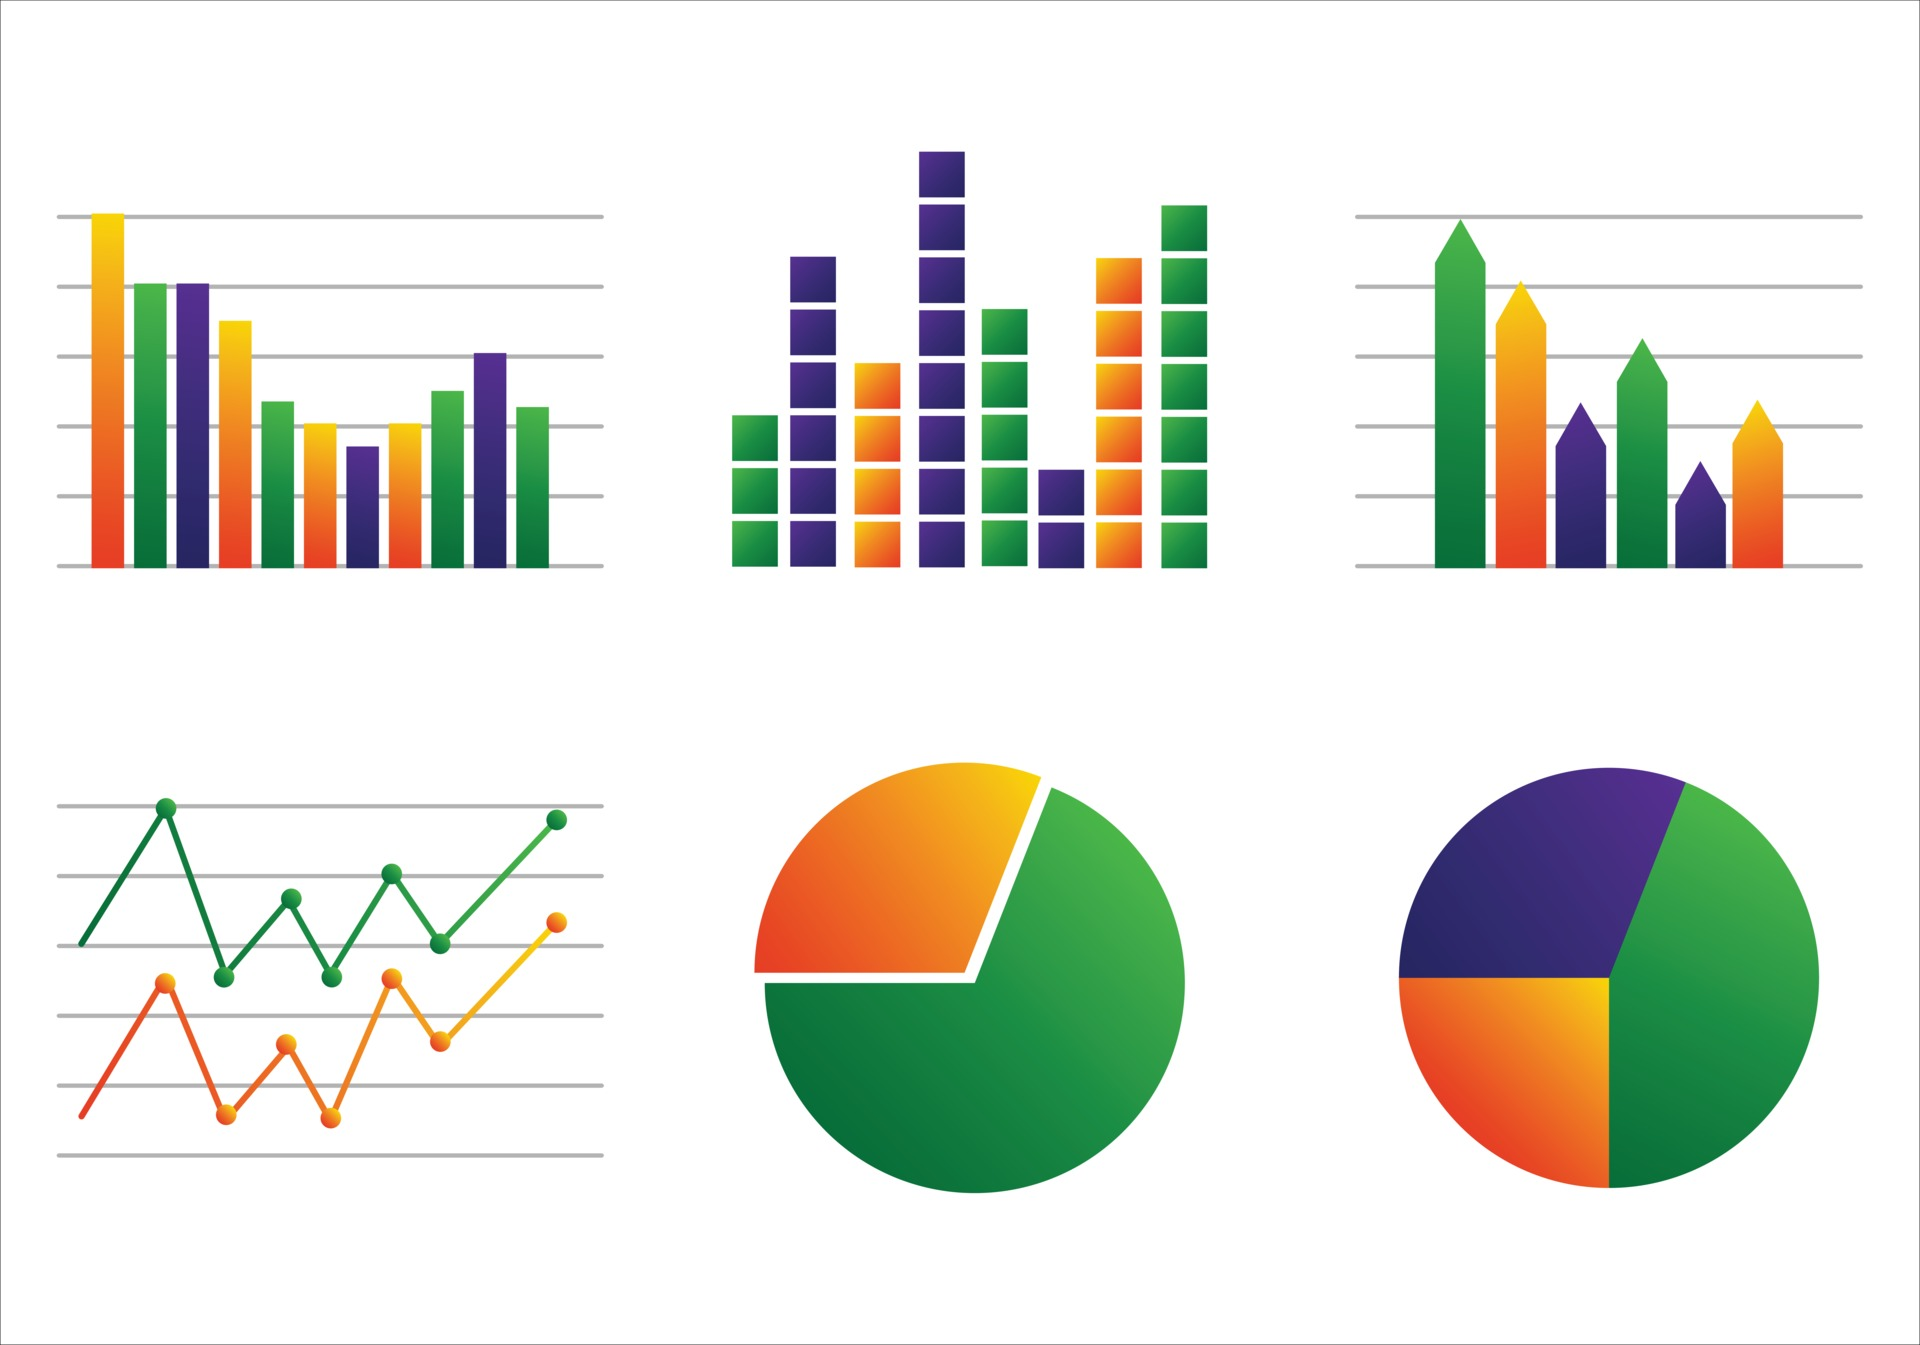
\includegraphics[width=0.8\linewidth]{graph}
\end{figure}
\blindtext

\blindtext

\blindtext
\begin{figure}[t]
\centering
\caption{Heading of the figure, with \texttt{[t]}}
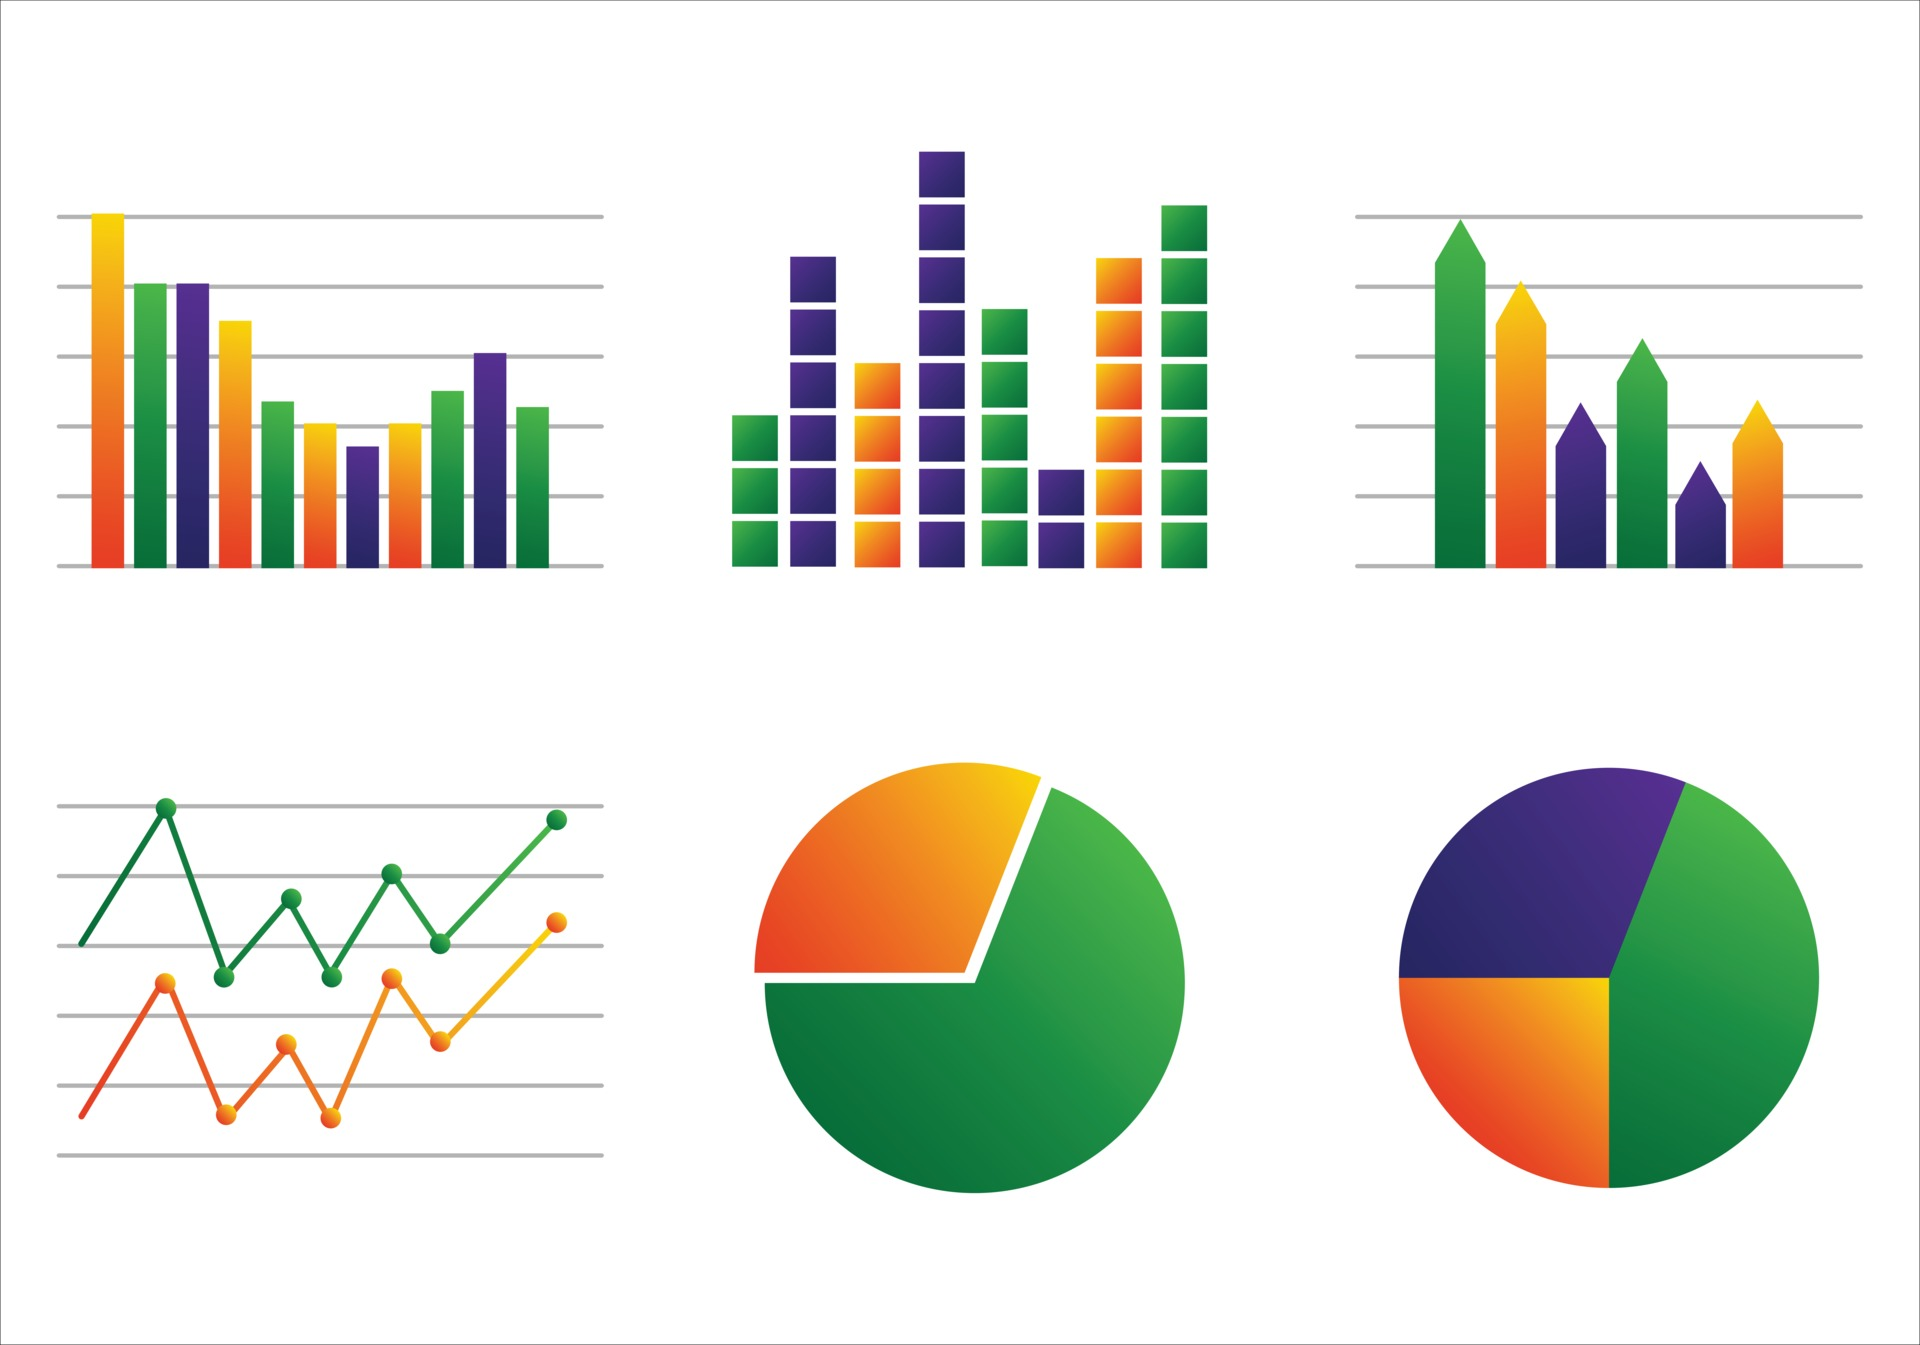
\includegraphics[width=0.8\linewidth]{graph}
\end{figure}
\blindtext


\blindtext
\begin{figure}[t]
\centering
\caption{Main heading of the figure, with \texttt{[t]}}
\begin{subfigure}{0.48\textwidth}
\caption{Heading of first figure}
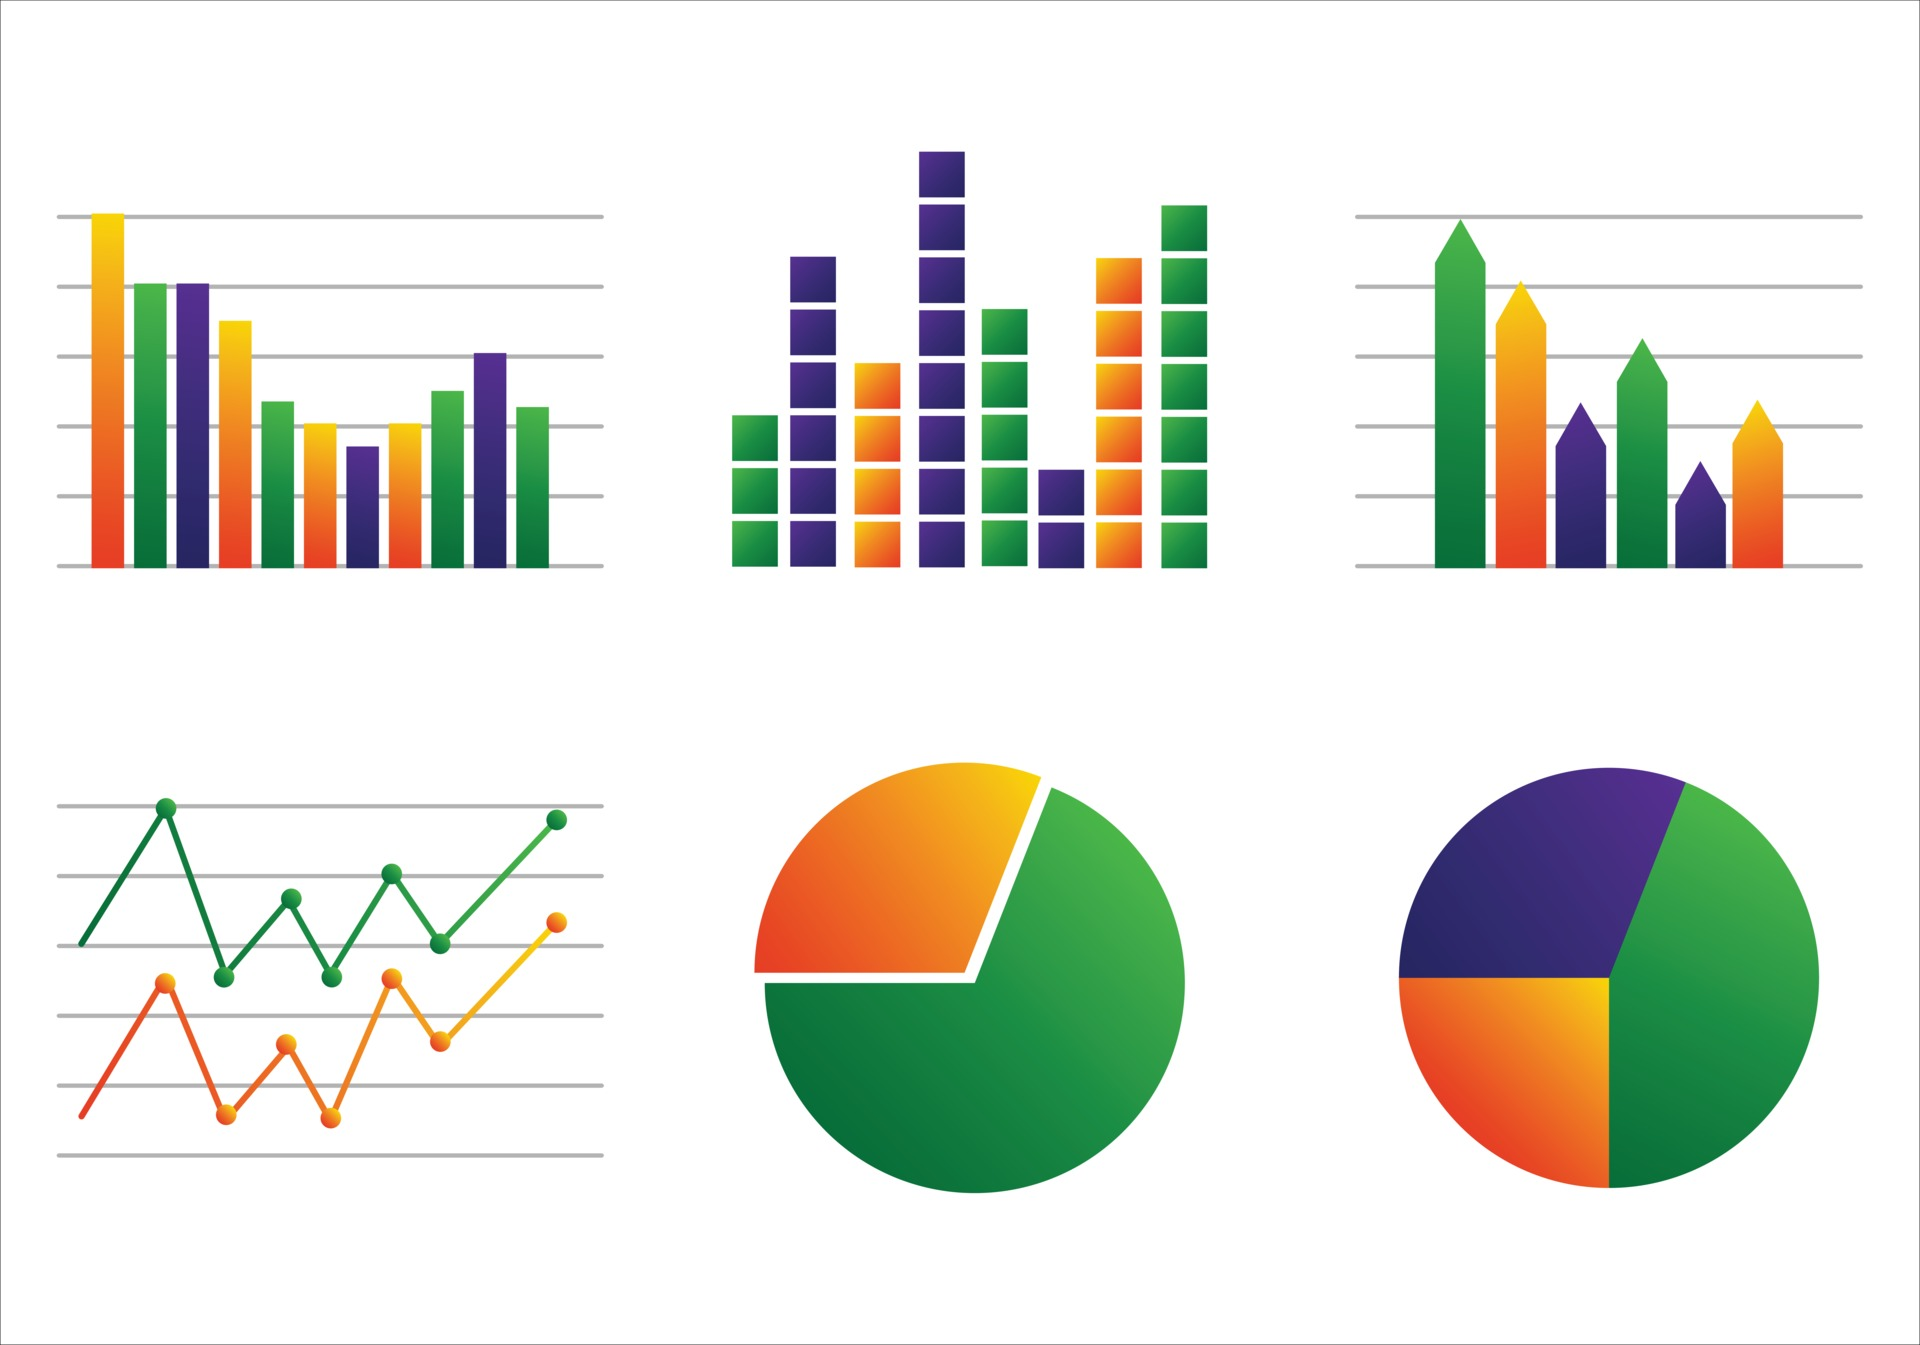
\includegraphics[width=1\linewidth]{graph}
\end{subfigure}
\begin{subfigure}{0.48\textwidth}
\caption{Heading of second figure}
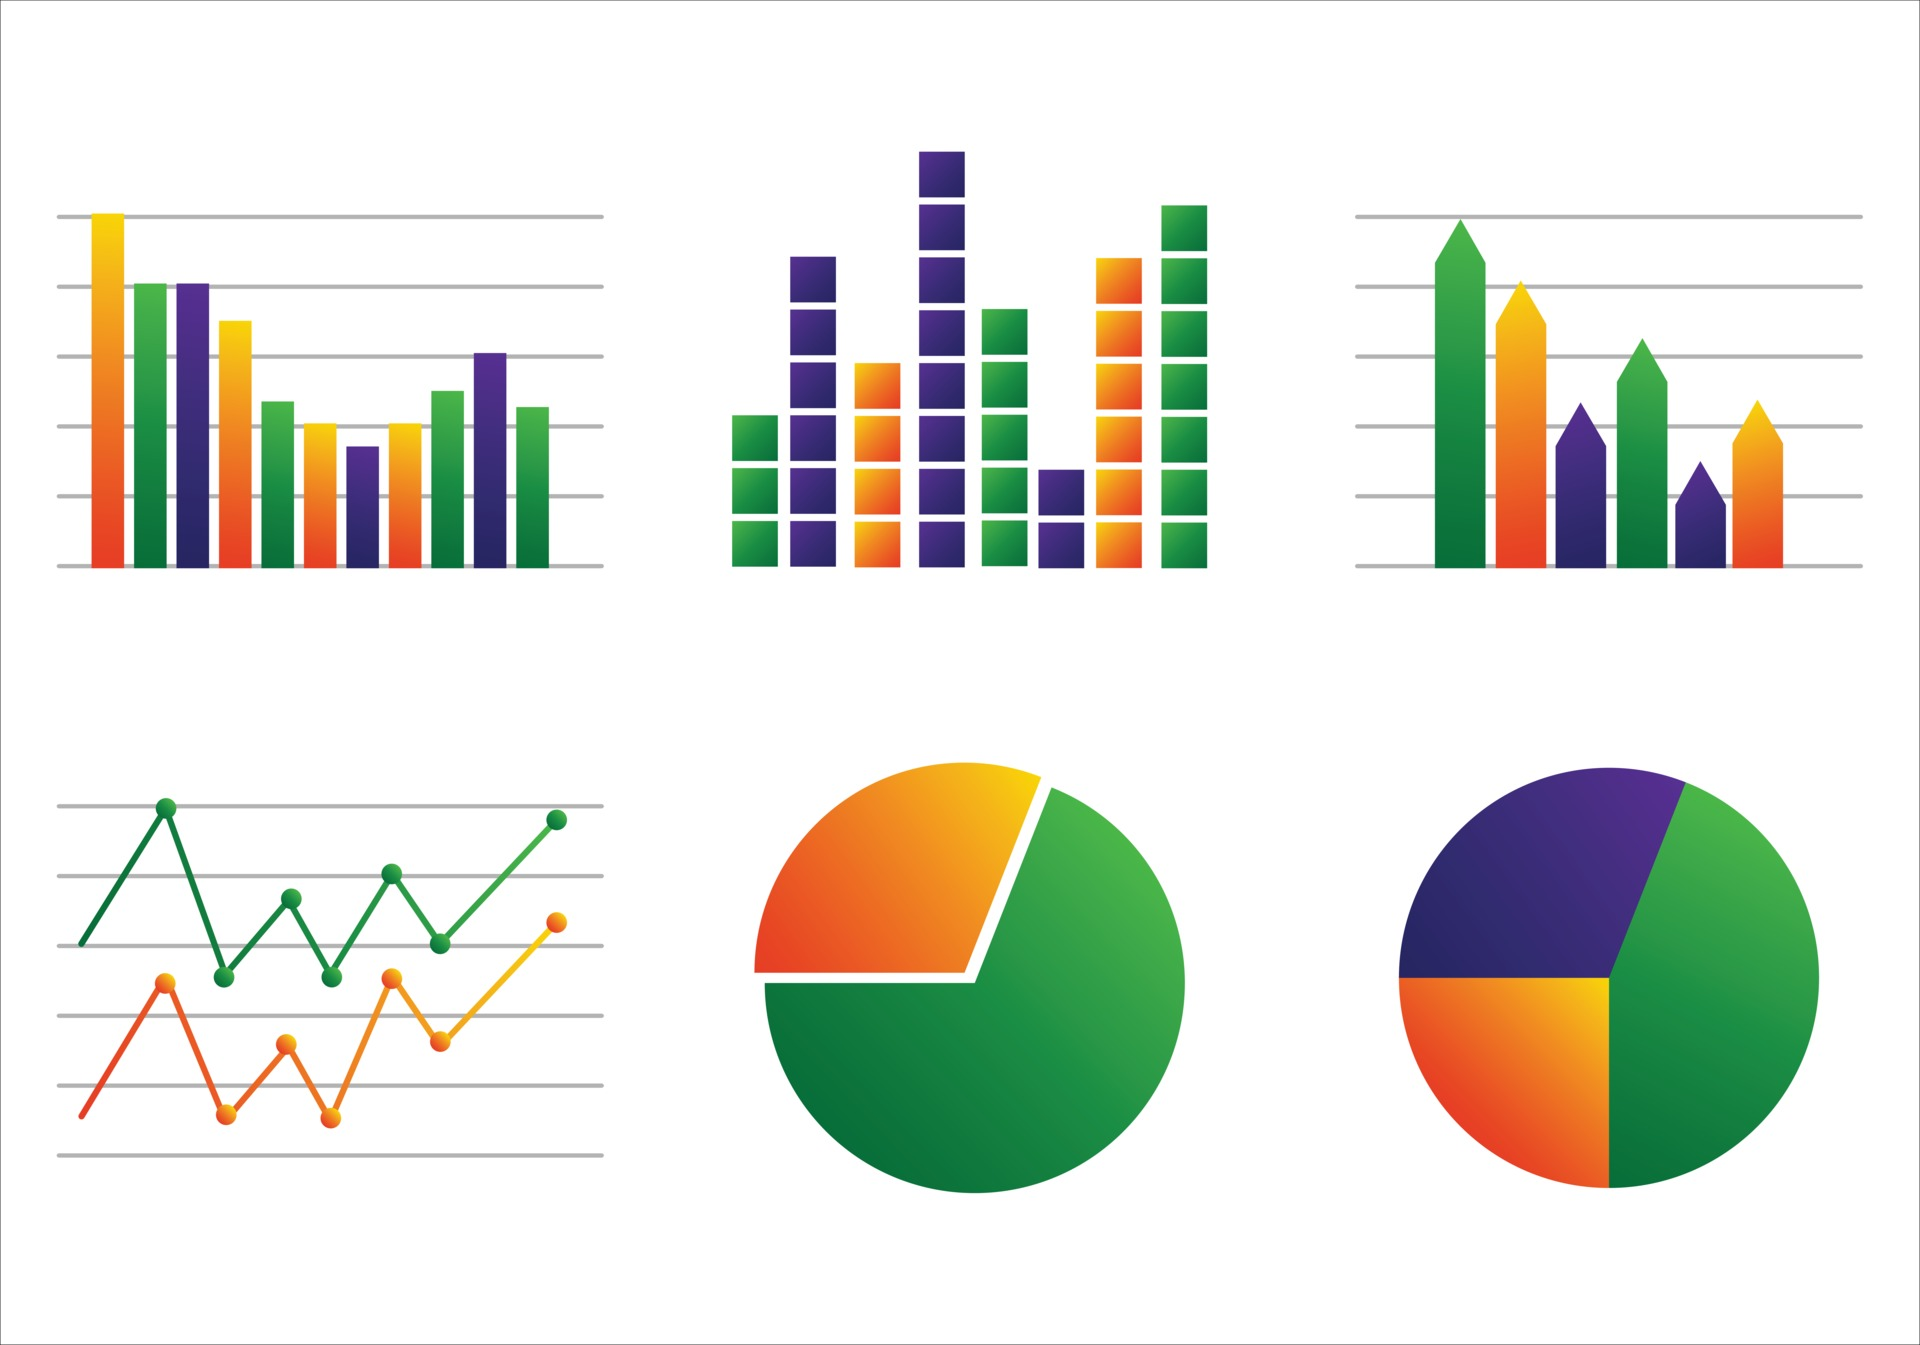
\includegraphics[width=1\linewidth]{graph}
\end{subfigure}
\end{figure}
\blindtext

%%%%%%%%%%%%%%%%%%%%%%%%%%%%%%%%%%%%%%%%%%

\end{document}
